%
% Manchester Raspberry Jam Workshop Booklet
%
% This template is designed to try and aide consistency between each booklet.
% Insert files and settings only as instructed by comments.
%

% Is this document PRINT or WEB format?
% use \printtrue or \printfalse
\newif\ifprint
\printtrue

% Page Formatting
\ifprint
	\documentclass[a4paper, twocolumn, twoside, 11pt]{article}
	\usepackage[margin=2cm]{geometry}
	\setlength{\columnsep}{1.25cm}
	\setlength{\parskip}{6pt}
\else
	\documentclass[a4paper, onecolumn, oneside, 11pt]{article}
	\usepackage[margin=3cm]{geometry}
	\setlength{\parskip}{9pt}
\fi



% FONT and text format
\usepackage[utf8x]{inputenc}	
\usepackage[UKenglish]{babel}
\ifprint
	\usepackage[usenames, dvipsnames]{color}				%Font Colour
	\usepackage[colorlinks=false]{hyperref}	%URLs
\else
	\usepackage[T1]{fontenc}
	\usepackage[sfdefault]{roboto}
	\usepackage[T1]{fontenc}
	\usepackage[usenames, dvipsnames]{color}				%Font Colour
	\usepackage[colorlinks=true,linkcolor=black,urlcolor=WildStrawberry]{hyperref}
\fi



% Table of Contents Format
\usepackage{tocloft}
\addtocontents{toc}{\cftpagenumbersoff{subsection}}
\setcounter{tocdepth}{2}
\setcounter{secnumdepth}{2}



% Section spacing
\ifprint
	\usepackage[compact]{titlesec}
\fi



% Listings and Asides
\usepackage{McrRaspJam/common/listings}
\usepackage{McrRaspJam/common/asides}



%Clear page for web version
\newcommand{\webclearpage}{
	\ifprint
	\else
		\clearpage
	\fi
}

% misc.
\usepackage{enumitem}									%List spacing changes
\usepackage[toc,page]{appendix}							%Appendix package
\usepackage{graphicx}									% TOC?
\usepackage{etoolbox}									%Boolean used for print/web switching
\usepackage{fancyvrb}									%Centered verbatim

% Enter the document title here
\newcommand{\workshopTitle}{Workshop 15: GPIO Zero}

% Enter the author of this workshop
\newcommand{\workshopAuthor}{Written by Jack Kelly}


\begin{document}
	% Title Format
\ifprint
	\title{Manchester Raspberry Jam \\ \workshopTitle}
	\author{}
\else
	\title{
		\begin{center}
			
\includegraphics[width=30mm]{McrRaspJam/common/logo-512}
		\end{center}
		\vspace{12pt}
		\workshopTitle
	}
	\author{
		Written by \workshopAuthor
	}
\fi

\date{\vspace{-16pt}}
\maketitle


% Online download location
\ifprint
	\begin{mdframed}[rightline=false, leftline=false]
		\scriptsize
		This booklet is available online at \mbox{\href{https://drive.google.com/open?id=0B_1SFjX_5JrmfnhpX0pPRXl6bmJNal8zdUxMeWZOdjJyZVdzU3V6UnBGdlVIMENtbFFkbVk}{bit.ly/McrRaspJam}}
		\normalsize
	\end{mdframed}
\fi
	
	%Place a SINGLE paragraph summary here
	Learn the basics of physical computing on Raspberry Pi using the \textit{GPIO Zero} Python library.
	
	%Difficulty
	\textit{Difficulty: Introductory workshop}
	
	\ifprint
		\renewcommand{\baselinestretch}{0.75}\normalsize
		\tableofcontents
		\renewcommand{\baselinestretch}{1.0}\normalsize
	\else
		\tableofcontents
	\fi
	
	%
	% Input the main CONTENT below, sans title page or contents.
	% Recommend inputting per section, and adding page breaks here.
	%
	% \webclearpage command is provided, will break page for web format only.
	%
	
	\setcounter{section}{-1}
\section{Introduction}

	If you've controlled electronics using the Raspberry Pi's GPIO before, you probably used a Python library called \textit{RPi.GPIO} to write your programs.
	
	GPIO Zero is an alternative GPIO library for Python, written by Raspberry Pi's Ben Nuttall, with the help of Dave Jones. It is designed to be easier to use than RPi.GPIO, whilst having the same capabilities.

	Today, we'll learn how to create simple breadboard circuits using the Raspberry Pi's GPIO, then we'll write Python programs that control those circuits using the GPIO Zero library.

	%Difficulty
	This is an introductory workshop, for people who have tried basic programming in Python before.
		
	\subsection*{How to use these booklets}

	The aim of these booklets is to help you attempt these workshops at home, and to explain concepts in more detail than at the workshop. You don't need to follow these booklets during the workshop, but you can if you'd like 0to.
	
	%Code Listings
		When you need to make changes to your code, they'll be presented in \textit{listings} like the example below. Some lines may be repeated across multiple listings, so check the line numbers to make sure you're not copying something twice.

	\lstinputlisting[style=Python, lastline=2]{McrRaspJam/015_GPIOZero/0_introduction/led.py}
	
	
	
	Occasionally, a concept will be explained in greater detail in \textit{asides}, like the one below. You can read these as you wish, but they're not required to complete the workshop.
	
\begin{aside}[Resistors]
	Resistors are most commonly used to limit the amount of current flowing through part of an electrical circuit.
	
	For example we use resistors in series with LEDs, as otherwise they could draw so much power that they destroy themselves.
	
	Buttons have almost no internal resistance, so we use high value ($\sim 10  k\Omega$) resistors to prevent current flowing straight from the power supply to ground; if we didn't, the entire CPU could be short circuited, and the Pi would lose power!
\end{aside}
	
	%\subsection*{What you'll need}
	
		% We'll be using Java for this workshop, which is installed by default in Raspbian.
	
	\subsection*{Everything else}
	
		% Aknowledgements
		These booklets were created using \textrm{\LaTeX}, an advanced typesetting system used for several sorts of books, academic reports and letters.
		\ifprint\else
			If you'd like to have a look at using LaTeX, We recommend looking at \TeX studio, which is available on most platforms, and also in the Raspbian repository.
		\fi
		
		
		% License spiel
		To allow modification and redistribution of these booklets, they are distributed under the \hbox{CC BY-SA 4.0} License.
		Latex source documents are available at \url{http://github.com/McrRaspJam/booklet-workshops}
		
		If you get stuck, find errors or have feedback about these booklets, please email me at:
		\href{mailto:jam@jackjkelly.com}{\texttt{jam@jackjkelly.com}}
	
	\clearpage
	\section{Creating a Simple Circuit}

We'll start with a very simple circuit. Let's build the circuit first, then we'll take a look at how it works afterwards.
	
	\webclearpage
	\section{Traffic Lights}

	\clearpage	
	\section{Morse Code Challenge}
	
	\clearpage	
	\begin{appendices}
		\section{Resistor Values}

	The resistance of axial through-hole resistors can be determined from the coloured bands printed on their exterior.
	
	A guide for 5-band resistors is shown below, depicting a $470 k\Omega$ resistor.
	
	\begin{center}
		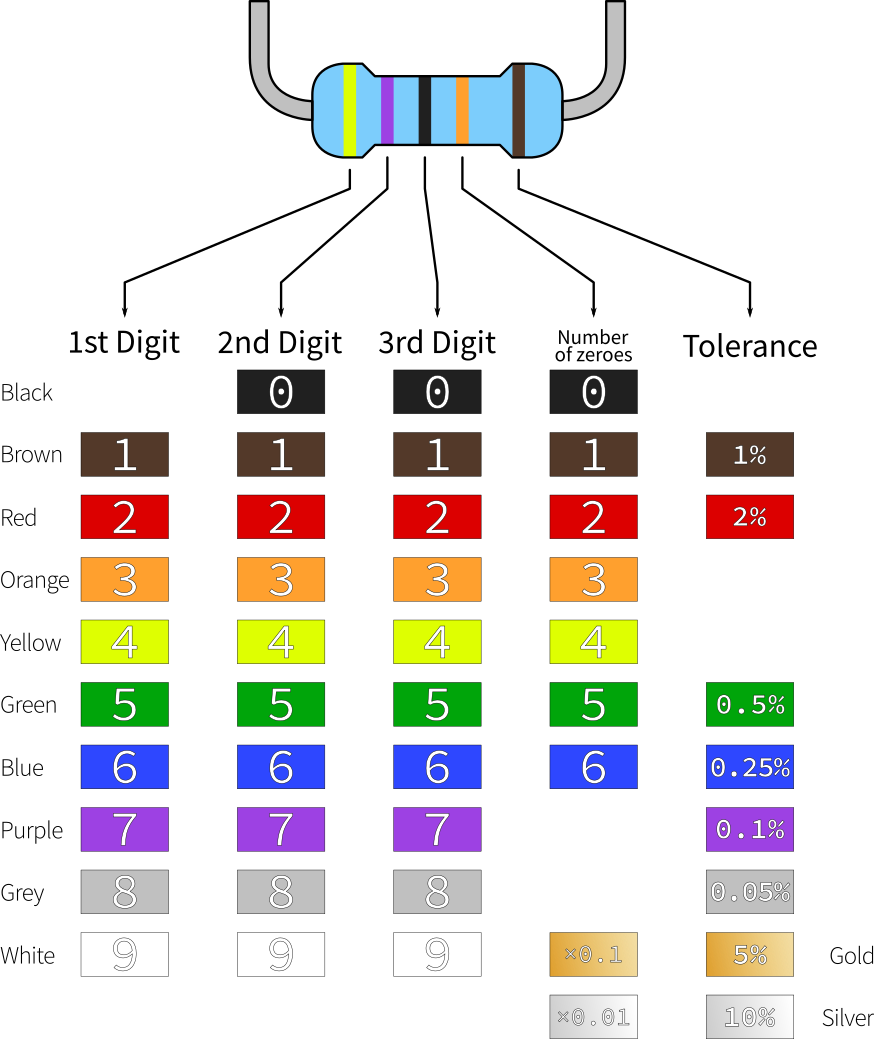
\includegraphics[width=0.7\linewidth]{McrRaspJam/015_GPIOZero/8_resistorbands/5band}
	\end{center}
		\webclearpage
		
		\section{International Morse Code}

\small

	\subsection*{Standard rules}
	
		\begin{itemize}[noitemsep]
			\item The length of a dot is 1 unit.
			\item The length of a dash is 3 units.
			\item The space between parts of the same letter is 1 unit.
			\item The space between letters is 3 units.
			\item The space between words is 7 units.
		\end{itemize}
	
	\subsection*{Beginner's rules}
	
		This rule-set is adjusted to make it easier to listen to and write down incoming Morse code messages. It's recommended that you write your morse code program to use these timings.
		
		\begin{itemize}[noitemsep]
			\item A unit is $\sim$\textbf{0.25} seconds.
			\item The length of a dot is 1 unit.
			\item The length of a dash is 4 units.
			\item The space between parts of the same letter is 1 unit.
			\item The space between letters is 8 units.
			\item The space between words is $\sim$20 units.
		\end{itemize}

	\subsection*{Characters}

	\subsubsection*{Alphabet}
	
		\begin{tabular}{rl}
			A & · − \\ 
			B & − · · · \\ 
			C & − · − ·  \\ 
			D & − · ·  \\ 
			E & ·  \\ 
			F & · · − ·  \\ 
			G & − − ·  \\ 
			H & · · · ·  \\ 
			I & · ·  \\ 
			J & · − − −  \\ 
			K & − · −  \\ 
			L & · − · ·  \\ 
			M & − −  \\ 
			N & − ·  \\ 
			O & − − −  \\
			P & · − − ·  \\
			Q & − − · −  \\ 
			R & · − ·  \\ 
			S & · · ·  \\ 
			T & −  \\ 
			U & · · −  \\ 
			V & · · · −  \\ 
			W & · − −  \\ 
			X & − · · −  \\ 
			Y & − · − −  \\ 
			Z & − − · ·  \\ 
		\end{tabular}
	
	\subsubsection*{Numeral}
	
		\begin{tabular}{rl}
			0 & − − − − − \\ 
			1 & · − − − − \\ 
			2 & · · − − − \\ 
			3 & · · · − − \\ 
			4 & · · · · − \\ 
			5 & · · · · · \\ 
			6 & − · · · · \\ 
			7 & − − · · · \\
			8 & − − − · · \\ 
			9 & − − − − · \\ 
		\end{tabular}
	
	\subsubsection*{Punctuation}
	
		\begin{tabular}{rl}
			. & · − · − · − \\ 
			, & − − · · − − \\ 
			? & · · − − · · \\ 
			! & − · − · − − \\ 
			( & − · − − · \\ 
			) & − · − − · − \\ 
			: & − − − · · · \\
			; & − · − · − · \\
			= & − · · · − \\ 
			+ & · − · − · \\
			- & − · · · · − \\ 
			'' & · − · · − · \\
			' & · − − − − · \\
		\end{tabular}\textbf{}
	
		\ifprint
		\else
			Additional ITU recognised characters exist, these can be found at \href{https://en.wikipedia.org/wiki/Morse_code#Letters.2C_numbers.2C_punctuation.2C_prosigns_for_Morse_code_and_non-English_variants}{\texttt{http://en.wikipedia.org/wiki/Morse\_code}}
		\fi

\iffalse

	\subsection*{Example Phrases}

		\begin{verbatim}
· · ·   − − −   · · ·
 S       O       S
		\end{verbatim}
		SOS

		\begin{verbatim}
· · · ·   ·   · − · ·   · − · ·   − − −
  H     E     L        L        O 
		\end{verbatim}
		Hello

		\begin{verbatim}
· − − − −   · · − − −       · · · − −
    1             2     SPACE     3
		\end{verbatim}
		12 3 (\textit{not} 1 2 3)

		\begin{verbatim}
· · ·   −   · − ·   − · − − ·   − · − − · −
 S     T     R         (             )
		\end{verbatim}
		str()
	
		\begin{verbatim}
· ·   − · · · −   · ·   · − · − ·   · − − − −
 I       =       I       +           1
		\end{verbatim}
		i = i+1

\fi

\normalsize

	\end{appendices}

\end{document}